% ===============================================
% Structural Obstruction Elimination via High-Dimensional Projection and Collapse Mechanisms
% ===============================================
\documentclass[11pt]{article}

% === Language and Font ===
\usepackage[utf8]{inputenc}       % UTF-8 input
\usepackage[T1]{fontenc}          % T1 font encoding
\usepackage{fontspec}             % XeLaTeX font support
\setmainfont{Times New Roman}     % Set main font

% === Math and Symbols ===
\usepackage{amsmath, amssymb, amsthm, amsfonts}
\usepackage{mathtools}
\usepackage{mathrsfs}
\usepackage{stmaryrd}             % For \llbracket etc.
\usepackage{bm}                   % Bold math symbols
\usepackage{changepage} 

% === TikZ and Diagrams ===
\usepackage{tikz}
\usepackage{tikz-cd}
\usetikzlibrary{
  cd, matrix, arrows.meta, decorations.pathmorphing, calc, positioning,
  decorations.markings, shapes.geometric
}

\usepackage{amscd} % Additional support for commutative diagrams

% === Listings for Coq, Code etc. ===
\usepackage{listings}
\usepackage{xcolor}
\usepackage{graphicx}             % For rotatebox, scalebox etc.
\usepackage{amsmath}
\usepackage{amssymb}


\lstdefinelanguage{Coq}{
  keywords={Definition,Theorem,Proof,Qed,Fixpoint,match,with,end,fun,let,in,forall,exists,Inductive,return,Type},
  keywordstyle=\color{blue}\bfseries,
  identifierstyle=\color{black},
  comment=[l]{//},
  commentstyle=\color{gray},
  morecomment=[s]{(*}{*)},
  string=[b]",
  stringstyle=\color{red},
}

\lstset{
  language=Coq,
  basicstyle=\ttfamily\footnotesize,
  keywordstyle=\color{blue},
  commentstyle=\color{gray},
  breaklines=true,
  breakindent=0pt,
  columns=flexible,
  keepspaces=true,
  xleftmargin=1em,
  framexrightmargin=1em,
  frame=single,
  captionpos=b
}

% === Geometry and Layout ===
\usepackage{geometry}
\geometry{margin=1in}
\usepackage{placeins}             % \FloatBarrier support

% === Hyperlinks ===
\usepackage[colorlinks=true, linkcolor=blue, citecolor=blue, urlcolor=blue]{hyperref}

% === Language Support ===
\usepackage[english]{babel}       % Use English language (place last)

% === Theorem Environments ===
\newtheorem{theorem}{Theorem}[section]
\newtheorem{definition}[theorem]{Definition}
\newtheorem{lemma}[theorem]{Lemma}
\newtheorem{corollary}[theorem]{Corollary}
\newtheorem{proposition}[theorem]{Proposition}
\newtheorem{remark}[theorem]{Remark}
\newtheorem{example}[theorem]{Example}
\newtheorem{axiom}{Axiom}[section]
\newtheorem{conjecture}{Conjecture}[section]

% === Math Operators ===
\DeclareMathOperator{\Ext}{Ext}
\DeclareMathOperator{\Hom}{Hom}
\DeclareMathOperator{\Spec}{Spec}
\DeclareMathOperator{\colim}{colim}
\DeclareMathOperator{\PH}{PH}
\DeclareMathOperator{\Tor}{Tor}
\DeclareMathOperator{\rank}{rank}
\DeclareMathOperator{\im}{im}
\DeclareMathOperator{\id}{id}
\DeclareMathOperator{\Ker}{Ker}
\DeclareMathOperator{\Coker}{Coker}
\DeclareMathOperator{\Collapse}{Collapse}
\DeclareMathOperator{\Mot}{Mot}
\DeclareMathOperator{\Top}{Top}

% === Custom Shortcuts ===
\newcommand{\QQ}{\mathbb{Q}}
\newcommand{\RR}{\mathbb{R}}
\newcommand{\CC}{\mathbb{C}}
\newcommand{\ZZ}{\mathbb{Z}}
\newcommand{\TT}{\mathbb{T}}

\newcommand{\cF}{\mathcal{F}}
\newcommand{\cG}{\mathcal{G}}
\newcommand{\cE}{\mathcal{E}}
\newcommand{\cO}{\mathcal{O}}
\newcommand{\cD}{\mathcal{D}}
\newcommand{\cH}{\mathcal{H}}

\newcommand{\into}{\hookrightarrow}
\newcommand{\onto}{\twoheadrightarrow}
\newcommand{\eps}{\varepsilon}
\newcommand{\Sha}{\mathcal{X}}

% === Document Metadata ===
\title{Structural Obstruction Elimination via High-Dimensional Projection and Collapse Mechanisms}
\author{Atsushi Kobayashi}
\date{}

\begin{document}

\maketitle


\begin{abstract}
We propose a structural-collapse framework utilizing high-dimensional projection and categorical collapse mechanisms to systematically eliminate topological and algebraic obstructions in mathematical structures. Our main contributions are: 
\begin{enumerate}
    \item Definition of high-dimensional lifting and degeneration processes that transform filtered objects into collapse-sheaves with trivial persistent homology (PH$_1$) and Ext$^1$-classes;
    \item Collapse functor formulation, establishing the equivalence 
    \[
    PH_1 = 0 \iff Ext^1 = 0 \implies \text{Group Collapse} \implies \text{Smoothness};
    \]
    \item Type-theoretic interpretation, providing a constructive criterion for smoothness detection in Coq/Lean-compatible terms;
    \item Structural comparison with existing approaches in persistent homology, homological algebra, and topological obstruction theory.
\end{enumerate}
This provides a unified and rigorous method to recognize and remove categorical obstructions, yielding smoothness and regularity across diverse mathematical contexts, particularly for algebraic, geometric, or analytic structures. While full extensions to motivic, Langlands, or mirror symmetry frameworks are beyond this paper's scope, we outline their potential as future developments. A preliminary preprint of this work (including broader structural extensions) is available at Zenodo: \url{https://doi.org/10.5281/zenodo.15743071}
\end{abstract}


\section{Introduction}

The systematic identification and elimination of structural obstructions remains a central challenge across diverse areas of mathematics, including topology, algebraic geometry, and category theory. Obstructions such as non-trivial topological cycles, extension classes, or complex group-theoretic structures often prevent desirable properties such as smoothness, regularity, or simplification from being achieved.

In recent years, advances in persistent homology, obstruction theory, and higher-categorical techniques have provided new tools for analyzing these phenomena. However, a unified framework that combines these approaches into a coherent method for detecting and eliminating obstructions has remained elusive.

The goal of this work is to propose a structural-collapse framework that integrates high-dimensional projection, degeneration analysis, and categorical collapse mechanisms to systematically address these challenges. Our approach formalizes how filtered mathematical structures can be lifted into higher-dimensional projection spaces, where obstructions become both visible and tractable. Through this process, persistent homology and Ext-class obstructions can be systematically addressed and, under suitable structural conditions, eliminated, enabling categorical and group-theoretic simplifications that lead to smoothness and regularity.

The main contributions of this paper are as follows:
\begin{itemize}
    \item We introduce the notion of high-dimensional projection and degeneration structures, providing a geometric and categorical setting in which obstructions can be systematically analyzed;
    \item We formalize the concept of a collapse functor that transforms filtered objects into collapse-sheaves characterized by the vanishing of persistent homology ($PH_1=0$) and extension classes ($Ext^1=0$);
    \item We demonstrate how this collapse process induces group-theoretic simplifications, such as the trivialization of Galois groups or fundamental groups;
    \item We provide a type-theoretic interpretation that encodes obstruction elimination and smoothness criteria in a formal, Coq/Lean-compatible framework;
    \item We compare this approach with existing methods in obstruction theory, persistent homology, and categorical simplification.
\end{itemize}

This work represents a focused presentation of the core components of a broader structural-collapse theory, emphasizing the foundational aspects relevant to obstruction elimination. A preliminary preprint, including extensions to motivic, Langlands, and mirror-symmetry frameworks, is available at Zenodo~\cite{ZenodoPreprint}.

The paper is organized as follows. In Section~2, we introduce the necessary mathematical preliminaries. Section~3 presents the structural-collapse framework. In Section~4, we provide the type-theoretic interpretation. Section~5 offers a structural comparison with existing approaches. Finally, in Section~6, we summarize our contributions and discuss future directions.


\section{Mathematical Preliminaries}

In this section, we summarize the mathematical background required to formulate our obstruction elimination framework. We adopt standard categorical, homological, and topological terminology throughout.

\subsection{Filtered Objects and High-Dimensional Projection}

Let $\mathcal{C}$ be a suitable mathematical category, such as that of topological spaces, algebraic varieties, or structured sheaves. We denote by $\mathsf{Filt}(\mathcal{C})$ the category of \emph{filtered objects}, equipped with a finite or persistent filtration reflecting geometric or algebraic complexity.

We introduce the concept of a \emph{high-dimensional projection}:
\[
\Pi : \mathsf{Filt}(\mathcal{C}) \longrightarrow \mathcal{P}(\mathcal{C}),
\]
where $\mathcal{P}(\mathcal{C})$ is a suitable higher-dimensional projection space, constructed to reveal hidden obstructions and degenerations within filtered objects. The precise structure of $\mathcal{P}(\mathcal{C})$ depends on the context, but it is assumed to admit degeneration processes and categorical simplifications.

\subsection{Persistent Homology and Ext-Class Obstructions}

We utilize persistent homology $\mathrm{PH}_1$ as a tool to detect topological obstructions in filtered objects. For $\mathcal{F} \in \mathsf{Filt}(\mathcal{C})$, $\mathrm{PH}_1(\mathcal{F})$ encodes first-order topological cycles that persist across the filtration.

In addition, we consider obstruction classes arising from homological algebra. For $\mathcal{F} \in \mathsf{Filt}(\mathcal{C})$ and a suitable coefficient system $\mathcal{G}$, the extension group $\mathrm{Ext}^1(\mathcal{F}, \mathcal{G})$ detects categorical and algebraic obstructions to trivialization.

\subsection{Collapse Functor and Collapse Sheaves}

We define the \emph{collapse functor}:
\[
C : \mathsf{Filt}(\mathcal{C}) \longrightarrow \mathsf{Triv}(\mathcal{C}),
\]
where $\mathsf{Triv}(\mathcal{C})$ denotes the category of \emph{collapse-sheaves}, characterized by:
\[
\mathrm{PH}_1(\mathcal{F}) = 0, \quad \mathrm{Ext}^1(\mathcal{F}, \mathcal{G}) = 0.
\]
Collapse-sheaves represent objects free of topological and categorical obstructions, suitable for further structural simplification.

\subsection{Group Collapse and Smoothness}

In many applications, objects in $\mathsf{Triv}(\mathcal{C})$ exhibit simplified group-theoretic structure. We use the term \emph{group collapse} to describe the trivialization or reduction of associated groups, such as Galois groups, fundamental groups, or automorphism groups.

Group collapse serves as a structural precursor to smoothness or regularity in the underlying mathematical objects. The precise implications are detailed in subsequent sections.


\subsection{Illustrative Diagram of High-Dimensional Projection}

To clarify the role of high-dimensional projection in obstruction elimination, we present a conceptual diagram illustrating the lifting and degeneration process.

\begin{figure}[h]
\centering
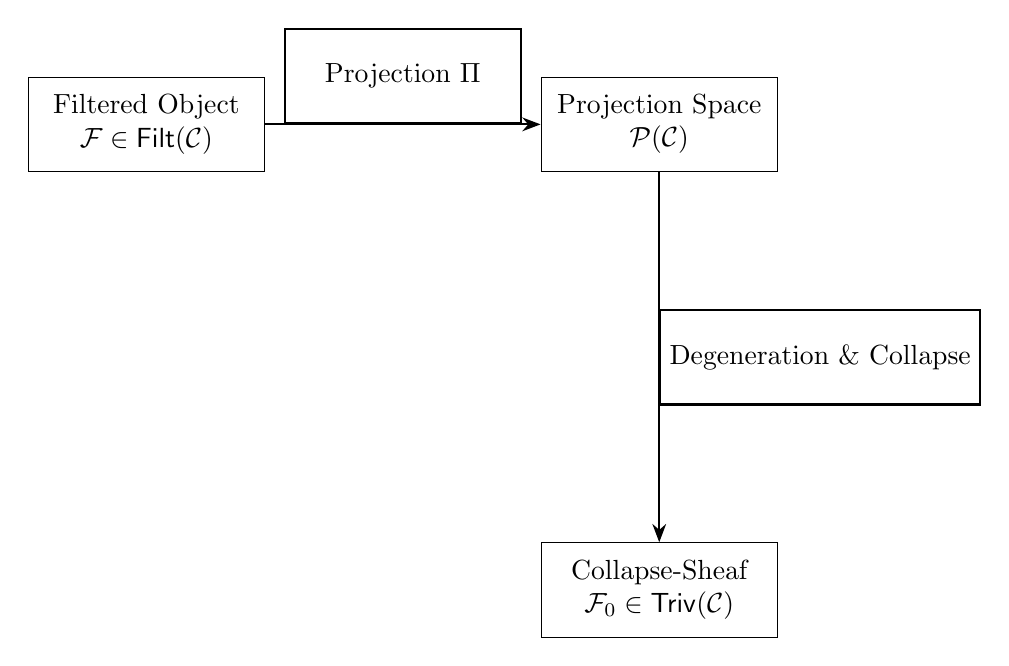
\begin{tikzpicture}[
    node distance=3.5cm, 
    every node/.style={draw, align=center, minimum width=3cm, minimum height=1.2cm},
    arrow/.style={-Stealth, thick}
]

% Nodes
\node (F) {Filtered Object\\ $\mathcal{F} \in \mathsf{Filt}(\mathcal{C})$};
\node (P) [right=of F] {Projection Space\\ $\mathcal{P}(\mathcal{C})$};
\node (T) [below=of P, yshift=-1.2cm] {Collapse-Sheaf\\ $\mathcal{F}_0 \in \mathsf{Triv}(\mathcal{C})$};

% Arrows
\draw[arrow] (F) -- node[above] {Projection $\Pi$} (P);
\draw[arrow] (P) -- node[right] {Degeneration \& Collapse} (T);

\end{tikzpicture}
\caption{High-dimensional projection and degeneration process. Hidden obstructions in $\mathcal{F}$ become visible after projection to $\mathcal{P}(\mathcal{C})$, enabling degeneration and collapse to a simplified structure $\mathcal{F}_0$.}
\label{fig:projection}
\end{figure}

Filtered objects $\mathcal{F} \in \mathsf{Filt}(\mathcal{C})$ may contain latent topological or algebraic obstructions that are difficult to analyze directly. The projection functor
\[
\Pi : \mathsf{Filt}(\mathcal{C}) \longrightarrow \mathcal{P}(\mathcal{C})
\]
lifts $\mathcal{F}$ into a higher-dimensional space $\mathcal{P}(\mathcal{C})$, designed to reveal hidden structures such as cycles, obstructions, or degeneration tendencies.

Degeneration processes within $\mathcal{P}(\mathcal{C})$ simplify the structure of $\mathcal{F}$, ultimately producing a collapse-sheaf $\mathcal{F}_0 \in \mathsf{Triv}(\mathcal{C})$, characterized by vanishing persistent homology and extension classes. This prepares the object for further structural simplification and smoothness realization.


\section{Collapse-Theoretic Framework}

We now formalize the obstruction elimination process through high-dimensional projection, categorical collapse, and group-theoretic simplification. This framework provides a unified structure for detecting and removing persistent topological and algebraic obstructions.

\subsection{Causal Structure of Obstruction Elimination}

The core logical structure of our framework is captured by the following causal chain, which holds under suitable structural conditions:
\[
\mathrm{PH}_1 = 0 \iff \mathrm{Ext}^1 = 0 \implies \text{Group Collapse} \implies \text{Smoothness}.
\]
Here, $\mathrm{PH}_1 = 0$ denotes the vanishing of persistent homology, eliminating first-order topological cycles. The equivalence $\mathrm{PH}_1 = 0 \iff \mathrm{Ext}^1 = 0$ reflects the structural correspondence between topological and categorical obstructions. Group collapse refers to the trivialization or reduction of associated groups, simplifying the global structure. Smoothness indicates the absence of residual singularities or irregularities.

\subsection{High-Dimensional Lifting and Degeneration}

Filtered objects $\mathcal{F} \in \mathsf{Filt}(\mathcal{C})$ are lifted via the projection functor:
\[
\Pi : \mathsf{Filt}(\mathcal{C}) \longrightarrow \mathcal{P}(\mathcal{C}),
\]
into a higher-dimensional projection space $\mathcal{P}(\mathcal{C})$. This space is designed to expose hidden obstructions and degeneration behavior.

Degeneration processes within $\mathcal{P}(\mathcal{C})$ simplify $\mathcal{F}$ by reducing its topological and categorical complexity, leading to the formation of collapse-sheaves in $\mathsf{Triv}(\mathcal{C})$.

\subsection{Collapse Functor and Obstruction Elimination}

The collapse functor $C : \mathsf{Filt}(\mathcal{C}) \to \mathsf{Triv}(\mathcal{C})$ acts by:

\begin{itemize}
    \item Eliminating persistent homology: $\mathrm{PH}_1(C(\mathcal{F})) = 0$;
    \item Trivializing extension classes: $\mathrm{Ext}^1(C(\mathcal{F}), \mathcal{G}) = 0$;
    \item Enabling group-theoretic simplification;
    \item Preparing the object for smoothness realization.
\end{itemize}

The collapse process combines topological, algebraic, and categorical operations into a coherent obstruction elimination mechanism.

\subsection{Implications and Applications}

This framework applies to a wide class of mathematical structures, including:

\begin{itemize}
    \item Topological spaces with persistent features;
    \item Algebraic or geometric objects exhibiting extension obstructions;
    \item Structures with complex group-theoretic properties (e.g., Galois groups, fundamental groups).
\end{itemize}

In subsequent sections, we refine this framework with type-theoretic formalization and structural comparison to existing approaches.


\subsection{Explicit Example of Collapse Functor}

We present a simplified topological example to illustrate the action of the collapse functor. Consider the category $\mathcal{C}$ of finite simplicial complexes. Let $\mathcal{F} \in \mathsf{Filt}(\mathcal{C})$ be a filtered simplicial complex containing a non-trivial first-order cycle, indicated by $\mathrm{PH}_1(\mathcal{F}) \neq 0$.

The collapse functor
\[
C : \mathsf{Filt}(\mathcal{C}) \longrightarrow \mathsf{Triv}(\mathcal{C})
\]
acts by eliminating such cycles and trivializing extension classes, yielding a collapse-sheaf $\mathcal{F}_0$ satisfying:
\[
\mathrm{PH}_1(\mathcal{F}_0) = 0, \quad \mathrm{Ext}^1(\mathcal{F}_0, \mathcal{G}) = 0.
\]

Figure~\ref{fig:collapse} provides a conceptual visualization of this process.

\begin{figure}[h]
\centering
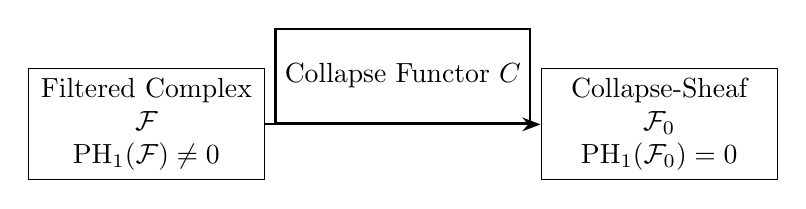
\begin{tikzpicture}[
    node distance=3.5cm, 
    every node/.style={draw, align=center, minimum width=3cm, minimum height=1.2cm},
    arrow/.style={-Stealth, thick}
]

% Nodes
\node (F) {Filtered Complex\\ $\mathcal{F}$ \\ $\mathrm{PH}_1(\mathcal{F}) \neq 0$};
\node (C) [right=of F] {Collapse-Sheaf\\ $\mathcal{F}_0$ \\ $\mathrm{PH}_1(\mathcal{F}_0) = 0$};

% Arrows
\draw[arrow] (F) -- node[above] {Collapse Functor $C$} (C);

\end{tikzpicture}
\caption{Schematic illustration of the collapse functor acting on a filtered simplicial complex. Non-trivial cycles in $\mathcal{F}$ are eliminated, producing a simplified collapse-sheaf $\mathcal{F}_0$.}
\label{fig:collapse}
\end{figure}

This toy example illustrates how the collapse framework operates concretely in a familiar topological setting. In more abstract categories, the same principles apply, with persistent homology and extension class obstructions eliminated through the collapse process.


\section{Type-Theoretic Interpretation}

To enhance the formal rigor and verifiability of the collapse framework, we provide a type-theoretic interpretation. This connects obstruction elimination to constructive logical systems, enabling formal reasoning and machine verification.

\subsection{Dependent Type Encoding of Collapse Conditions}

We employ dependent type theory to express obstruction elimination conditions. Let $\mathcal{F} \in \mathsf{Filt}(\mathcal{C})$ be a filtered object. The collapse conditions are encoded as:

\[
\prod_{\mathcal{F} : \mathsf{Filt}(\mathcal{C})} 
\left( \mathrm{PH}_1(\mathcal{F}) = 0 \rightarrow \mathrm{Ext}^1(\mathcal{F}, \mathcal{G}) = 0 \right),
\]

where $\prod$ denotes the dependent product type, formalizing the implication from vanishing persistent homology to the trivialization of extension classes. This expresses the elimination of both topological and categorical obstructions in a machine-verifiable form.

\subsection{Collapse Process as Type-Theoretic Chain}

The full collapse process can be encoded in type-theoretic terms as:

\[
\prod_{\mathcal{F} : \mathsf{Filt}(\mathcal{C})} 
\left( 
\mathrm{PH}_1(\mathcal{F}) = 0 \rightarrow \mathrm{Ext}^1(\mathcal{F}, \mathcal{G}) = 0 
\rightarrow \text{Group Collapse}(\mathcal{F}) 
\rightarrow \text{Smoothness}(\mathcal{F})
\right).
\]

This chain reflects the logical structure of obstruction elimination within a constructive formal system.


\subsection{Coq/Lean Encoding Snippet}

To demonstrate the formal verifiability of the collapse framework, we provide a simple Coq-style encoding of the logical structure. This encoding expresses the causal chain of obstruction elimination as machine-verifiable propositions.

\begin{lstlisting}[language=Coq]
Parameter PH1_trivial : Prop.
Parameter Ext1_trivial : Prop.
Parameter Group_collapse : Prop.
Parameter Smoothness : Prop.

Axiom CollapseChain :
  PH1_trivial <-> Ext1_trivial ->
  Group_collapse ->
  Smoothness.
\end{lstlisting}

Figure~\ref{fig:typechain} presents a conceptual visualization of the corresponding logical dependencies.

\begin{figure}[h]
\centering
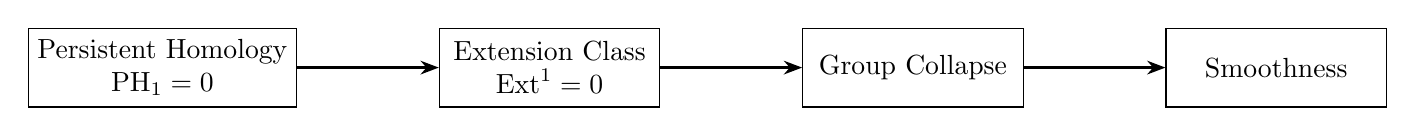
\begin{tikzpicture}[
    node distance=1.8cm, 
    every node/.style={draw, align=center, minimum width=2.8cm, minimum height=1cm},
    arrow/.style={-Stealth, thick}
]

% Nodes
\node (PH) {Persistent Homology\\ $\mathrm{PH}_1 = 0$};
\node (Ext) [right=of PH] {Extension Class\\ $\mathrm{Ext}^1 = 0$};
\node (Grp) [right=of Ext] {Group Collapse};
\node (Sm) [right=of Grp] {Smoothness};

% Arrows
\draw[arrow] (PH) -- (Ext);
\draw[arrow] (Ext) -- (Grp);
\draw[arrow] (Grp) -- (Sm);

\end{tikzpicture}
\caption{Logical structure of the collapse chain. Vanishing persistent homology implies trivial extension classes, enabling group-theoretic collapse and leading to smoothness realization.}
\label{fig:typechain}
\end{figure}

The encoding aligns with the logical dependencies depicted in Figure~\ref{fig:typechain}, providing a formal foundation for implementing the collapse framework within proof assistants such as Coq or Lean.


\subsection{Formalization and Verifiability}

The type-theoretic interpretation aligns with formal proof assistants such as Coq or Lean. Collapse conditions can be encoded as propositions and verified within these systems, providing:

\begin{itemize}
    \item Formal logical structure to obstruction elimination;
    \item Machine-verifiable criteria for smoothness;
    \item This may provide avenues for exploring connections with homotopy type theory and higher-categorical logic.
\end{itemize}

This enhances both the mathematical rigor and practical verifiability of the collapse framework.

The type-theoretic interpretation aligns with formal proof assistants such as Coq or Lean~\cite{CoqManual2017}. 
This may provide avenues for exploring connections with homotopy type theory and higher-categorical logic~\cite{HOTT2013}.


\section{Structural Comparison with Existing Approaches}

In this section, we compare the proposed collapse-theoretic framework with existing methods for analyzing and eliminating structural obstructions in mathematics. Our goal is to clarify the scope, novelty, and limitations of the present work.

\subsection{Persistent Homology and Topological Simplification}

Persistent homology has been widely utilized to detect and analyze topological features that persist across filtrations, particularly in applied topology and data analysis \cite{Edelsbrunner2008}. While persistent homology effectively reveals topological complexity, it does not inherently provide mechanisms for obstruction elimination or structural simplification.

In contrast, the collapse framework integrates persistent homology into a broader categorical and algebraic structure, where the vanishing of $\mathrm{PH}_1$ triggers a cascade of obstruction eliminations.

\subsection{Ext-Class Obstructions and Homological Algebra}

Obstructions arising from extension classes, such as $\mathrm{Ext}^1$, are well-studied in homological algebra and related fields \cite{Weibel1994}. Traditional approaches focus on computing or classifying these classes, often in specific algebraic or geometric contexts.

The collapse framework treats $\mathrm{Ext}^1$-class vanishing as an integral component of obstruction elimination, linked directly to topological simplification and group-theoretic collapse.

\subsection{Group-Theoretic Simplification}

Group-theoretic structures, including Galois groups, fundamental groups, and automorphism groups, often encode global obstructions to simplification or smoothness. Various methods exist for analyzing these groups, such as profinite methods or étale fundamental group techniques.

Our approach complements these methods by providing a structural process—the collapse chain—where group-theoretic simplification naturally follows from topological and categorical obstruction elimination.

Group collapse serves as a structural precursor to smoothness or regularity in the underlying mathematical objects.
The relationship between group collapse and cohomological structures parallels classical approaches such as Galois cohomology~\cite{Serre1997}.


\subsection{Positioning and Novelty of the Collapse Framework}

The collapse framework complements and extends aspects of existing approaches in persistent homology, homological algebra, and group-theoretic methods, while remaining compatible with their insights.

\begin{itemize}
    \item Providing a unified structure that connects topological, categorical, and group-theoretic obstruction elimination;
    \item Introducing high-dimensional projection and degeneration processes to reveal hidden complexity;
    \item Formalizing the obstruction elimination process within a type-theoretic and machine-verifiable setting;
    \item Extending beyond existing approaches in persistent homology, homological algebra, and group-theoretic methods, while remaining compatible with their insights.
\end{itemize}

Nevertheless, the framework presented here is intentionally focused on foundational aspects. Full extensions to motivic, Langlands, or mirror-symmetry structures are beyond the scope of this paper and will be addressed in future work.

Full extensions to motivic, Langlands, or mirror-symmetry structures~\cite{MirrorSymmetry2003} are beyond the scope of this paper and will be addressed in future work.



\subsection{Simplified Application Scenario}

While this paper focuses on the theoretical foundations of the collapse framework, we briefly outline a conceptual application illustrating how obstruction elimination may facilitate structural simplification and smoothness in a practical setting.

Consider a time-dependent vector field $u(t)$ defined on a domain $\Omega \subset \mathbb{R}^3$, governed by a partial differential equation (PDE) of the form:
\[
\partial_t u + (u \cdot \nabla)u = -\nabla p + \nu \Delta u, \quad \nabla \cdot u = 0,
\]
which structurally resembles the incompressible Navier-Stokes equations. In complex fluid systems, topological structures such as persistent vortices or singularities may emerge, obstructing smoothness and regularity.

By associating a filtered object $\mathcal{F}(t) \in \mathsf{Filt}(\mathcal{C})$ encoding the topological and categorical features of $u(t)$, the collapse framework can be applied:
\begin{itemize}
    \item The projection functor $\Pi$ lifts $\mathcal{F}(t)$ to a higher-dimensional space, exposing hidden obstructions;
    \item Degeneration and collapse processes eliminate these obstructions, producing a collapse-sheaf $\mathcal{F}_0(t)$;
    \item The resulting structure simplifies group-theoretic complexity and enables smoothness of $u(t)$.
\end{itemize}

This scenario suggests a structural pathway by which collapse-theoretic methods may contribute to understanding or achieving global regularity in PDE systems. A rigorous, fully formal development of such applications lies beyond the scope of this paper and will be pursued in future work.


\section{Conclusion and Future Directions}

We have presented a structural-collapse framework that integrates high-dimensional projection, degeneration analysis, and categorical collapse mechanisms to systematically eliminate topological and algebraic obstructions. The framework establishes a unified causal structure in which the vanishing of persistent homology ($\mathrm{PH}_1=0$) implies the trivialization of extension classes ($\mathrm{Ext}^1=0$), leading to group-theoretic simplification and, ultimately, smoothness realization.

Through formalization within a type-theoretic and categorical setting, the collapse framework enhances both the structural understanding and formal verifiability of obstruction phenomena. Illustrative examples in Sections 3.5 and 5.5 demonstrate the conceptual applicability of the framework to simplified topological settings and potential PDE applications.

Several important directions remain for future research:

\begin{itemize}
    \item Extending the collapse framework to motivic, Langlands, and mirror-symmetry structures, exploring the role of obstruction elimination in these broader contexts;
    \item Investigating rigorous connections to homotopy type theory and higher-categorical foundations;
    \item Developing detailed applications to concrete problems in algebraic geometry, topology, and number theory;
    \item Pursuing formal verification and implementation of collapse conditions within proof assistants such as Coq or Lean;
    \item Exploring the implications of collapse-theoretic methods for global regularity problems in partial differential equations, including the Navier-Stokes equations.
\end{itemize}

These directions represent promising avenues for further integrating structural-collapse methods into the broader mathematical landscape. The foundational contributions of this work aim to provide a rigorous basis for these future developments.



\begin{thebibliography}{99}

\bibitem{Edelsbrunner2008}
H.~Edelsbrunner and J.~Harer, \emph{Persistent homology---a survey}, 
Contemporary Mathematics, vol.~453, pp.~257--282, 2008.

\bibitem{Weibel1994}
C.~A. Weibel, \emph{An Introduction to Homological Algebra}, 
Cambridge University Press, 1994.

\bibitem{ZenodoPreprint}
A.~Kobayashi, \emph{Structural Obstruction Elimination via High-Dimensional Projection and Collapse Mechanisms}, Zenodo, 2024.\\
\texttt{https://doi.org/10.5281/zenodo.15743071}

\bibitem{HOTT2013}
The Univalent Foundations Program, \emph{Homotopy Type Theory: Univalent Foundations of Mathematics}, Institute for Advanced Study, 2013.

\bibitem{CoqManual2017}
B.~Barras et al., \emph{The Coq Proof Assistant Reference Manual}, INRIA, 2017.

\bibitem{Serre1997}
J.-P.~Serre, \emph{Galois Cohomology}, Springer, 1997.

\bibitem{MirrorSymmetry2003}
K.~Hori et al., \emph{Mirror Symmetry}, Clay Mathematics Monographs, 2003.


\end{thebibliography}


\end{document}
